\usetikzlibrary{patterns}
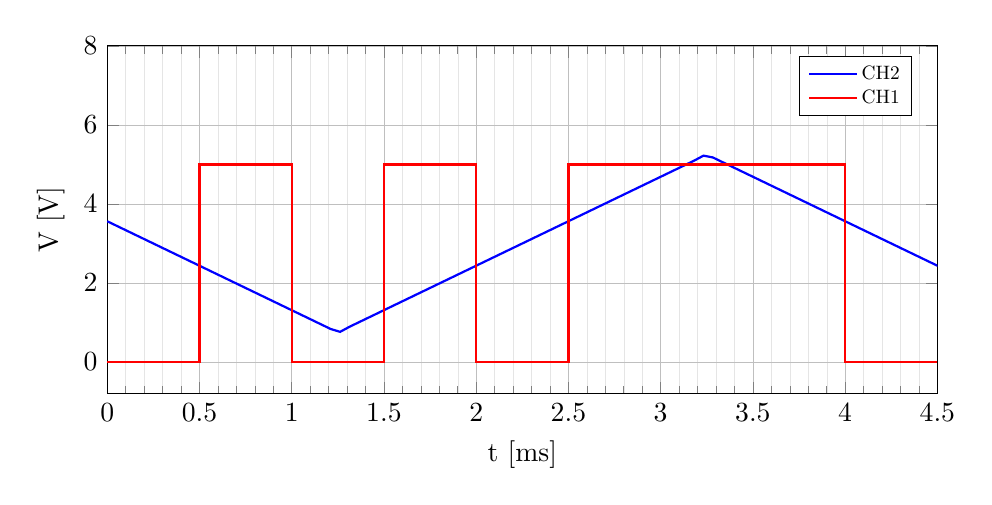
\begin{tikzpicture}
    \begin{axis}[
        width=\textwidth,
        height=6cm,
        grid=both,
        major grid style={line width=.2pt,draw=gray!50},
        minor grid style={line width=.1pt,draw=gray!20},
        xmin=0, xmax=4.5,
        ymax=8,
        xlabel={t [ms]},
        ylabel={V [V]},
        minor x tick num=4,
        legend pos=north east,
        legend style={nodes={scale=0.7, transform shape}}
    ]
        % Canal 1: Triangular 4Vpp, 200Hz (T=5ms)
        \addplot[blue, thick, domain=0:5, samples=100] {
            3 - (2 * 2.25 / pi) * rad(asin(sin(deg((pi/2) * (\x - 0.25)))))
        };
        \addlegendentry{CH2}

        % Canal 2: Tren de Pulsos (Burst)
        \addplot[red, thick] coordinates {
            (0,0) (0.5,0) (0.5, 5) (1, 5) (1, 0) (1.5, 0) (1.5, 5) (2, 5) (2, 0) (2.5, 0) (2.5, 5) (4, 5)
            (4, 0) (4.5, 0)};
        \addlegendentry{CH1}
    \end{axis}
\end{tikzpicture}
